% (C) Savoir-faire Linux, 2017 
% authored by Marc Lijour, March 2017
% Some art belong to their respective authors, as indicated in the document
% 
% Variables
% TODO set the variables
% ---------------------- USER-DEFINED --------------------------------
\newcommand{\SFLtitle}{FinTech Industry Outlook}
\newcommand{\SFLlongtitle}{FinTech Industry Outlook, Ryerson University}
\newcommand{\SFLsubtitle}{Trends, Case Study, and App Development Worshop (Liferay + Vaadin + Java)}
\newcommand{\SFLauthor}{Marc~Lijour}
\newcommand{\SFLdate}{March 15, 2017}
\newcommand{\SFLsubject}{Liferay in FinTech}
% --------------------------------------------------------------------
% Template
% (C) Savoir-faire Linux, 2016 (this document and associated logos and art)
% This document is licensed under a Creative Commons License BY-SA (feel free to use the code, but all rights are reserved for logos and art)
% https://creativecommons.org/licenses/by-sa/2.5/ca/
% Savoir-faire Linux presentation template for LaTeX
% authored by Marc Lijour, December 2016
% This template comes with a first page on a blue background
% Possible improvement in future iterations
% - Test and fix as needed to work on xetex (to use Ubuntu fonts)
% === USAGE===
% Create a file for your LaTeX content (slides, etc), in which you must do the following:
% TODO 1 - set variables defined below
% TODO 2 - include this code by calling: % (C) Savoir-faire Linux, 2016 (this document and associated logos and art)
% This document is licensed under a Creative Commons License BY-SA (feel free to use the code, but all rights are reserved for logos and art)
% https://creativecommons.org/licenses/by-sa/2.5/ca/
% Savoir-faire Linux presentation template for LaTeX
% authored by Marc Lijour, December 2016
% This template comes with a first page on a blue background
% Possible improvement in future iterations
% - Test and fix as needed to work on xetex (to use Ubuntu fonts)
% === USAGE===
% Create a file for your LaTeX content (slides, etc), in which you must do the following:
% TODO 1 - set variables defined below
% TODO 2 - include this code by calling: % (C) Savoir-faire Linux, 2016 (this document and associated logos and art)
% This document is licensed under a Creative Commons License BY-SA (feel free to use the code, but all rights are reserved for logos and art)
% https://creativecommons.org/licenses/by-sa/2.5/ca/
% Savoir-faire Linux presentation template for LaTeX
% authored by Marc Lijour, December 2016
% This template comes with a first page on a blue background
% Possible improvement in future iterations
% - Test and fix as needed to work on xetex (to use Ubuntu fonts)
% === USAGE===
% Create a file for your LaTeX content (slides, etc), in which you must do the following:
% TODO 1 - set variables defined below
% TODO 2 - include this code by calling: \input{sfl-presentation-template-blue-EN}
% TODO 3 - Start the document as usual and you're in business; just use \begin{document} and don't forget to conclude with \end{document}
% TODO 4 - Use the custom method \SFLcoverpage instead of \titlepage to create your cover page
% Voilà!
%
\documentclass{beamer}
\usepackage{etoolbox}
% Variables
% ---------------------- USER-DEFINED --------------------------------
\ifdef{\SFLtitle}{}{\newcommand{\SFLtitle}{\color{red}Title TBD}}
\ifdef{\SFLlongtitle}{}{\newcommand{\SFLlongtitle}{\color{red}Long title TBD}}
\ifdef{\SFLsubtitle}{}{\newcommand{\SFLsubtitle}{\color{red}Subtitle TBD}}
\ifdef{\SFLauthor}{}{\newcommand{\SFLauthor}{\color{red}Author TBD}}
\ifdef{\SFLdate}{}{\newcommand{\SFLdate}{\color{red}Date TBD}}
\ifdef{\SFLsubject}{}{\newcommand{\SFLsubject}{\color{red}Subject TBD}}
% --------------------------------------------------------------------
\usetheme{Boadilla}
% Set color close to Savoir-faire Linux standard
\definecolor{beamer@blendedblue}{RGB}{86,176,201}
% Cover Page
\title[\SFLtitle] {\SFLlongtitle}
\subtitle{\SFLsubtitle}
\author{\SFLauthor}
\date{\SFLdate}
\subject{\SFLsubject}
\usepackage{tikz}
% -- possible approach through modif of the template (abandonned for now)
%\addtobeamertemplate{title page}{
%    \tikz[remember picture,overlay]
%        \node at ([xshift=0cm,yshift=0cm]current page.center) 
%		 {
\includegraphics[width=\paperwidth, height=\paperheight]{./images/sfl-background-blue}};
%}{}
%\setbeamercolor{title page}{fg=white}
%\setbeamercolor{titlelike}{fg=white}
%\setbeamertemplate{navigation symbols}{}
% Try Xetex to use system fonts (pdflatex makes it hard to import a font)
%\usepackage{fontspec}
%\setsansfont{Ubuntu}
%\setmonofont{Ubuntu Mono}
%
%\usepackage[absolute,overlay]{textpos}
%\setlength{\TPHorizModule}{\paperwidth}
%\setlength{\TPVertModule}{\paperheight}
% -- create a custom (command) title page -which has the benefit of not affecting the settings for the rest of the presentation
\newcommand{\SFLcoverpage}{\frame[plain]{
	\tikz[remember picture,overlay] {
        	\node(bkgd) at ([xshift=0cm,yshift=0cm]current page.center) 
			{
\includegraphics[width=\paperwidth, height=\paperheight]{../templates/images/sfl-background-blue}};
        	\node(logo) at ([xshift=0cm,yshift=2.5cm]current page.center) 
		 	{
\includegraphics[scale=.20]{../templates/images/logo-sfl-blanc-rgb-72dpi}};
	}
	\tikz[remember picture,overlay] {
        	\node(title) at ([xshift=0cm,yshift=1cm]current page.center) 
			{\Large\color{white}\textbf{{\SFLlongtitle}}};
        	\node(subtitle) at ([xshift=0cm,yshift=.2cm]current page.center) 
			{\small\color{white}\emph{\SFLsubtitle}};
        	\node(author) at ([xshift=0cm,yshift=-2cm]current page.center) 
			{\small\color{white}By~\SFLauthor};
        	\node(date) at ([xshift=0cm,yshift=-2.5cm]current page.center) 
			{\tiny\color{white}\SFLdate};
        	\node(footnote) at ([xshift=0cm,yshift=-4cm]current page.center) 
			{\TINY\color{white}\emph{The registered trademark Linux$^\circledR$ is used pursuant to a sublicense from LMI, the exclusive licensee of Linus Torvalds, owner of the mark on a world-wide basis.}};
    	}
}}
%
% This sets a Savoir-faire Linux logo at the bottom right corner of each page
\logo{
\includegraphics[scale=.1]{../templates/images/logo-sfl-250.png}}
\AtBeginSection[]
{
  \begin{frame}
    \frametitle{Table of Contents}
    \tableofcontents[currentsection]
  \end{frame}
}
%\usepackage[format=plain,justification=raggedright,singlelinecheck=false]{caption}
\usepackage[format=plain,justification=justified,singlelinecheck=false]{caption}
\usepackage[utf8]{inputenc}
\usepackage{dirtytalk}
\usepackage{wrapfig}
\usepackage{hyperref}
\usepackage{verbatim}
\usepackage{mathabx}
%\usepackage{MnSymbol}


% TODO 3 - Start the document as usual and you're in business; just use \begin{document} and don't forget to conclude with \end{document}
% TODO 4 - Use the custom method \SFLcoverpage instead of \titlepage to create your cover page
% Voilà!
%
\documentclass{beamer}
\usepackage{etoolbox}
% Variables
% ---------------------- USER-DEFINED --------------------------------
\ifdef{\SFLtitle}{}{\newcommand{\SFLtitle}{\color{red}Title TBD}}
\ifdef{\SFLlongtitle}{}{\newcommand{\SFLlongtitle}{\color{red}Long title TBD}}
\ifdef{\SFLsubtitle}{}{\newcommand{\SFLsubtitle}{\color{red}Subtitle TBD}}
\ifdef{\SFLauthor}{}{\newcommand{\SFLauthor}{\color{red}Author TBD}}
\ifdef{\SFLdate}{}{\newcommand{\SFLdate}{\color{red}Date TBD}}
\ifdef{\SFLsubject}{}{\newcommand{\SFLsubject}{\color{red}Subject TBD}}
% --------------------------------------------------------------------
\usetheme{Boadilla}
% Set color close to Savoir-faire Linux standard
\definecolor{beamer@blendedblue}{RGB}{86,176,201}
% Cover Page
\title[\SFLtitle] {\SFLlongtitle}
\subtitle{\SFLsubtitle}
\author{\SFLauthor}
\date{\SFLdate}
\subject{\SFLsubject}
\usepackage{tikz}
% -- possible approach through modif of the template (abandonned for now)
%\addtobeamertemplate{title page}{
%    \tikz[remember picture,overlay]
%        \node at ([xshift=0cm,yshift=0cm]current page.center) 
%		 {
\includegraphics[width=\paperwidth, height=\paperheight]{./images/sfl-background-blue}};
%}{}
%\setbeamercolor{title page}{fg=white}
%\setbeamercolor{titlelike}{fg=white}
%\setbeamertemplate{navigation symbols}{}
% Try Xetex to use system fonts (pdflatex makes it hard to import a font)
%\usepackage{fontspec}
%\setsansfont{Ubuntu}
%\setmonofont{Ubuntu Mono}
%
%\usepackage[absolute,overlay]{textpos}
%\setlength{\TPHorizModule}{\paperwidth}
%\setlength{\TPVertModule}{\paperheight}
% -- create a custom (command) title page -which has the benefit of not affecting the settings for the rest of the presentation
\newcommand{\SFLcoverpage}{\frame[plain]{
	\tikz[remember picture,overlay] {
        	\node(bkgd) at ([xshift=0cm,yshift=0cm]current page.center) 
			{
\includegraphics[width=\paperwidth, height=\paperheight]{../templates/images/sfl-background-blue}};
        	\node(logo) at ([xshift=0cm,yshift=2.5cm]current page.center) 
		 	{
\includegraphics[scale=.20]{../templates/images/logo-sfl-blanc-rgb-72dpi}};
	}
	\tikz[remember picture,overlay] {
        	\node(title) at ([xshift=0cm,yshift=1cm]current page.center) 
			{\Large\color{white}\textbf{{\SFLlongtitle}}};
        	\node(subtitle) at ([xshift=0cm,yshift=.2cm]current page.center) 
			{\small\color{white}\emph{\SFLsubtitle}};
        	\node(author) at ([xshift=0cm,yshift=-2cm]current page.center) 
			{\small\color{white}By~\SFLauthor};
        	\node(date) at ([xshift=0cm,yshift=-2.5cm]current page.center) 
			{\tiny\color{white}\SFLdate};
        	\node(footnote) at ([xshift=0cm,yshift=-4cm]current page.center) 
			{\TINY\color{white}\emph{The registered trademark Linux$^\circledR$ is used pursuant to a sublicense from LMI, the exclusive licensee of Linus Torvalds, owner of the mark on a world-wide basis.}};
    	}
}}
%
% This sets a Savoir-faire Linux logo at the bottom right corner of each page
\logo{
\includegraphics[scale=.1]{../templates/images/logo-sfl-250.png}}
\AtBeginSection[]
{
  \begin{frame}
    \frametitle{Table of Contents}
    \tableofcontents[currentsection]
  \end{frame}
}
%\usepackage[format=plain,justification=raggedright,singlelinecheck=false]{caption}
\usepackage[format=plain,justification=justified,singlelinecheck=false]{caption}
\usepackage[utf8]{inputenc}
\usepackage{dirtytalk}
\usepackage{wrapfig}
\usepackage{hyperref}
\usepackage{verbatim}
\usepackage{mathabx}
%\usepackage{MnSymbol}


% TODO 3 - Start the document as usual and you're in business; just use \begin{document} and don't forget to conclude with \end{document}
% TODO 4 - Use the custom method \SFLcoverpage instead of \titlepage to create your cover page
% Voilà!
%
\documentclass{beamer}
\usepackage{etoolbox}
% Variables
% ---------------------- USER-DEFINED --------------------------------
\ifdef{\SFLtitle}{}{\newcommand{\SFLtitle}{\color{red}Title TBD}}
\ifdef{\SFLlongtitle}{}{\newcommand{\SFLlongtitle}{\color{red}Long title TBD}}
\ifdef{\SFLsubtitle}{}{\newcommand{\SFLsubtitle}{\color{red}Subtitle TBD}}
\ifdef{\SFLauthor}{}{\newcommand{\SFLauthor}{\color{red}Author TBD}}
\ifdef{\SFLdate}{}{\newcommand{\SFLdate}{\color{red}Date TBD}}
\ifdef{\SFLsubject}{}{\newcommand{\SFLsubject}{\color{red}Subject TBD}}
% --------------------------------------------------------------------
\usetheme{Boadilla}
% Set color close to Savoir-faire Linux standard
\definecolor{beamer@blendedblue}{RGB}{86,176,201}
% Cover Page
\title[\SFLtitle] {\SFLlongtitle}
\subtitle{\SFLsubtitle}
\author{\SFLauthor}
\date{\SFLdate}
\subject{\SFLsubject}
\usepackage{tikz}
% -- possible approach through modif of the template (abandonned for now)
%\addtobeamertemplate{title page}{
%    \tikz[remember picture,overlay]
%        \node at ([xshift=0cm,yshift=0cm]current page.center) 
%		 {
\includegraphics[width=\paperwidth, height=\paperheight]{./images/sfl-background-blue}};
%}{}
%\setbeamercolor{title page}{fg=white}
%\setbeamercolor{titlelike}{fg=white}
%\setbeamertemplate{navigation symbols}{}
% Try Xetex to use system fonts (pdflatex makes it hard to import a font)
%\usepackage{fontspec}
%\setsansfont{Ubuntu}
%\setmonofont{Ubuntu Mono}
%
%\usepackage[absolute,overlay]{textpos}
%\setlength{\TPHorizModule}{\paperwidth}
%\setlength{\TPVertModule}{\paperheight}
% -- create a custom (command) title page -which has the benefit of not affecting the settings for the rest of the presentation
\newcommand{\SFLcoverpage}{\frame[plain]{
	\tikz[remember picture,overlay] {
        	\node(bkgd) at ([xshift=0cm,yshift=0cm]current page.center) 
			{
\includegraphics[width=\paperwidth, height=\paperheight]{../../Savoir-faire_Linux-LaTeX_Templates/images/sfl-background-blue-non-interlaced}};
        	\node(logo) at ([xshift=0cm,yshift=2.5cm]current page.center) 
		 	{
\includegraphics[scale=.20]{../../Savoir-faire_Linux-LaTeX_Templates/images/logo-sfl-blanc-rgb-72dpi}};
	}
	\tikz[remember picture,overlay] {
        	\node(title) at ([xshift=0cm,yshift=1cm]current page.center) 
			{\Large\color{white}\textbf{{\SFLlongtitle}}};
        	\node(subtitle) at ([xshift=0cm,yshift=.2cm]current page.center) 
			{\small\color{white}\emph{\SFLsubtitle}};
        	\node(author) at ([xshift=0cm,yshift=-2cm]current page.center) 
			{\small\color{white}By~\SFLauthor};
        	\node(date) at ([xshift=0cm,yshift=-2.5cm]current page.center) 
			{\tiny\color{white}\SFLdate};
        	\node(footnote) at ([xshift=0cm,yshift=-4cm]current page.center) 
			{\TINY\color{white}\emph{The registered trademark Linux$^\circledR$ is used pursuant to a sublicense from LMI, the exclusive licensee of Linus Torvalds, owner of the mark on a world-wide basis.}};
    	}
}}
%
% This sets a Savoir-faire Linux logo at the bottom right corner of each page
\logo{
\includegraphics[scale=.1]{../../Savoir-faire_Linux-LaTeX_Templates/images/logo-sfl-250.png}}
\AtBeginSection[]
{
  \begin{frame}
    \frametitle{Table of Contents}
    \tableofcontents[currentsection]
  \end{frame}
}
%\usepackage[format=plain,justification=raggedright,singlelinecheck=false]{caption}
\usepackage[format=plain,justification=justified,singlelinecheck=false]{caption}
\usepackage[utf8]{inputenc}
\usepackage{dirtytalk}
\usepackage{wrapfig}
\usepackage{hyperref}
\usepackage{verbatim}
\usepackage{mathabx}
%\usepackage{MnSymbol}


% Extra packages
\usepackage{amssymb}
\usepackage{amsmath}
\usepackage[american]{babel}
\usepackage{csquotes}
%\usepackage[backend=biber,style=apa]{biblatex}
%\DeclareLanguageMapping{american}{american-apa}
% Use one bib file per section
%\addbibresource{references-program-overview.bib}
\definecolor{links}{HTML}{2A1B81}
\hypersetup{colorlinks,linkcolor=,urlcolor=links}
% Start of the document
\begin{document}
% Cover page
% Do not use this: \frame{\titlepage}
% use this instead:
\SFLcoverpage

% (C) Savoir-faire Linux, 2017 
% authored by Marc Lijour, March 2017 
% Some art belong to their respective authors, as indicated in the document
% 
% ======================================================================================================
%                                     OVERVIEW OF SAVOIR-FAIRE LINUX
% ======================================================================================================
\section{Who are we?}
% First big picture
\frame{
        \tikz[remember picture,overlay] {
                \node(bkgd) at ([xshift=0cm,yshift=.3cm]current page.center)
                        {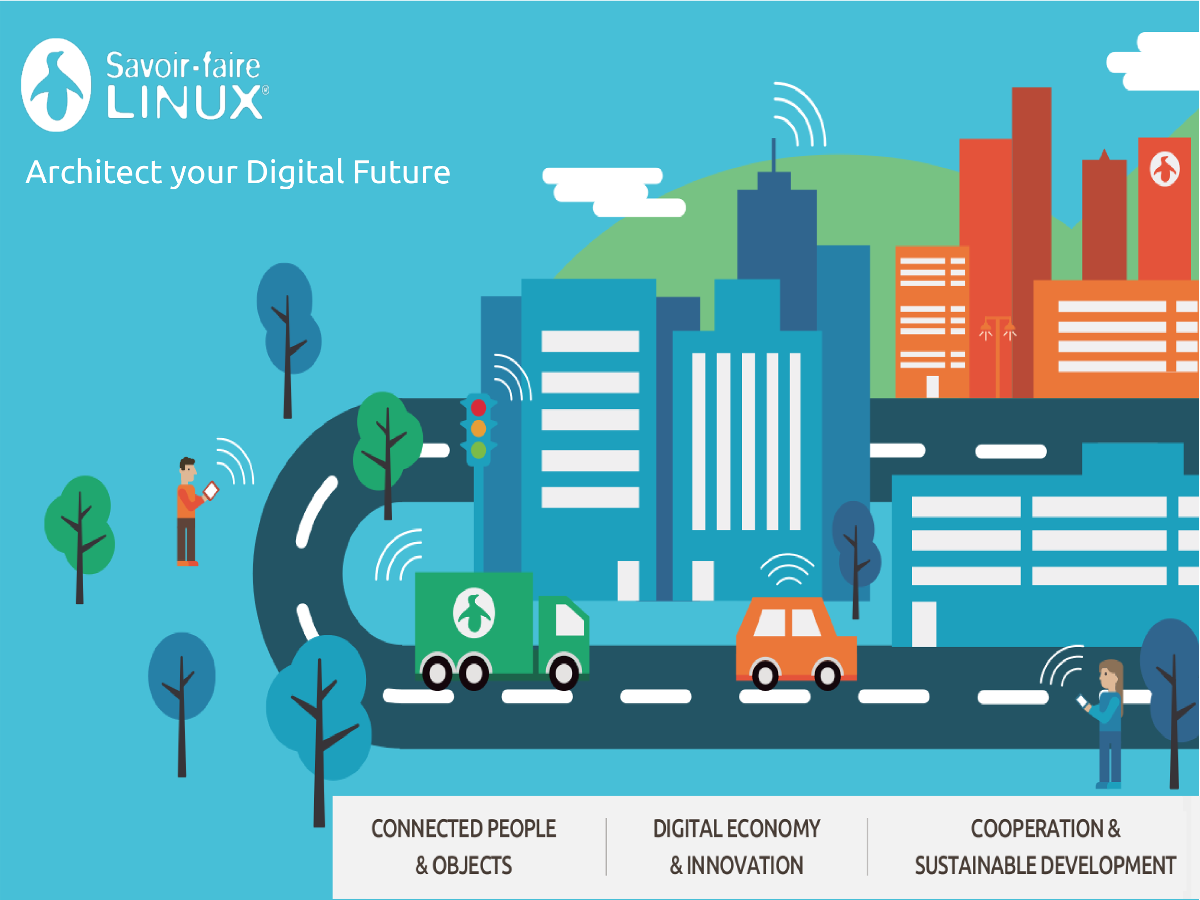
\includegraphics[width=\paperwidth]{../pics/SFL-architect-your-digital-future-128x96-non-interlaced}};
        }
}

\begin{frame}
	\frametitle{Company Profile}
	\begin{figure}
		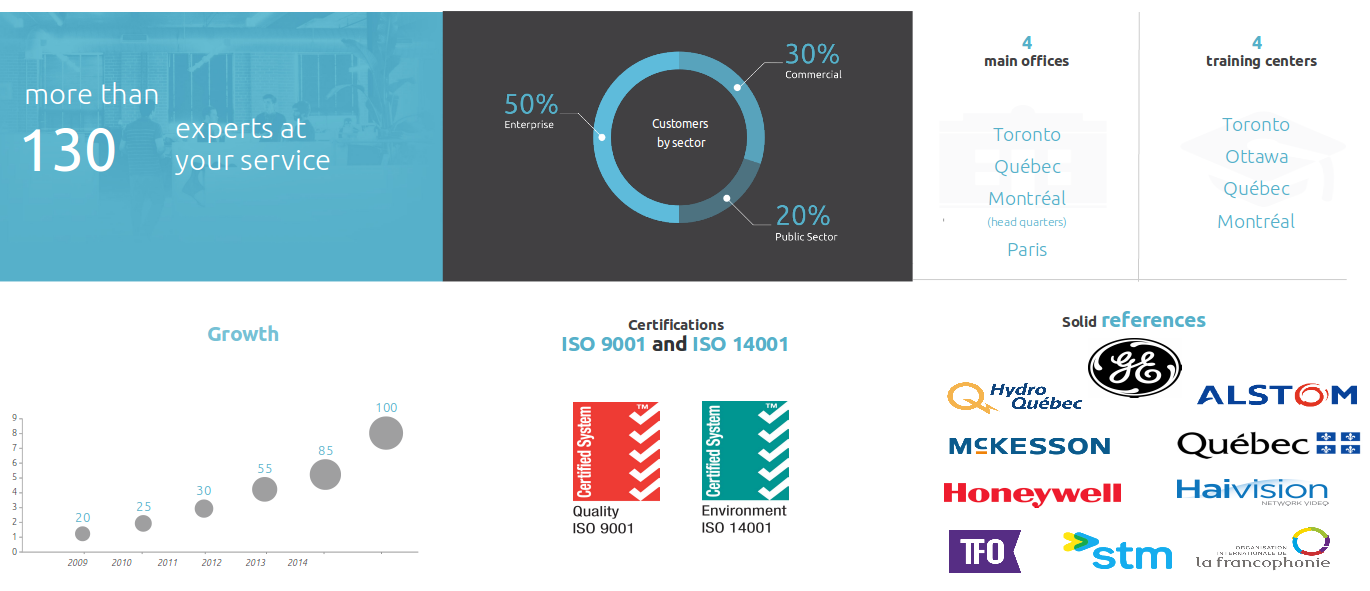
\includegraphics[width=11cm]{../pics/SFL-offices-customers}
	\end{figure}
\end{frame}

\begin{frame}
	\frametitle{A wide spectrum of competencies}
	\begin{figure}
		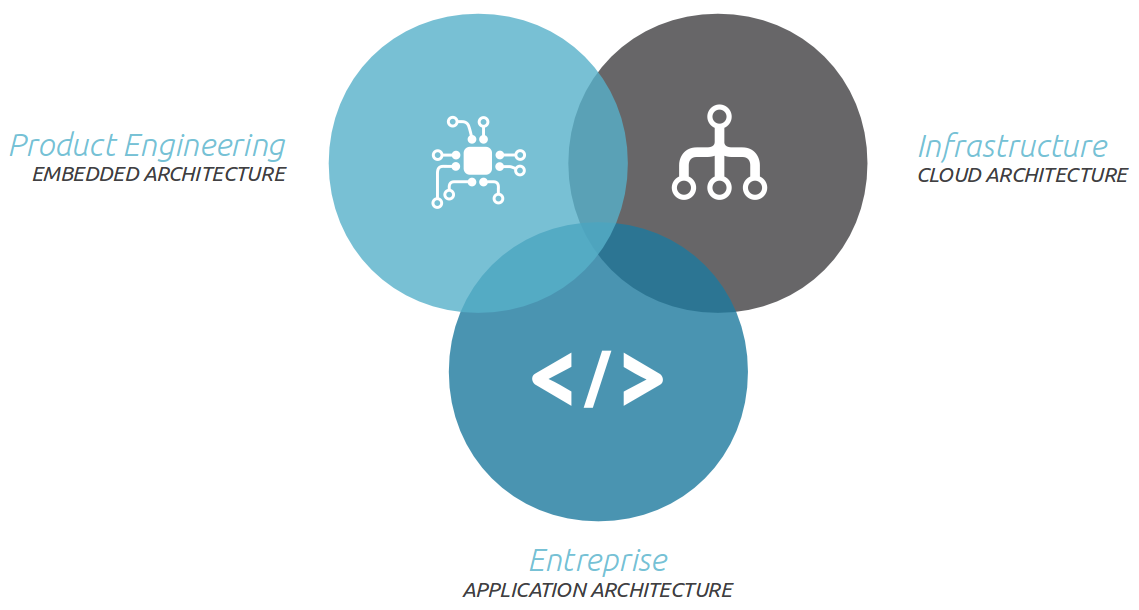
\includegraphics[width=11cm]{../pics/SFL-3-areas}
	\end{figure}
\end{frame}

\begin{frame}
	\frametitle{Services}
	\begin{figure}
		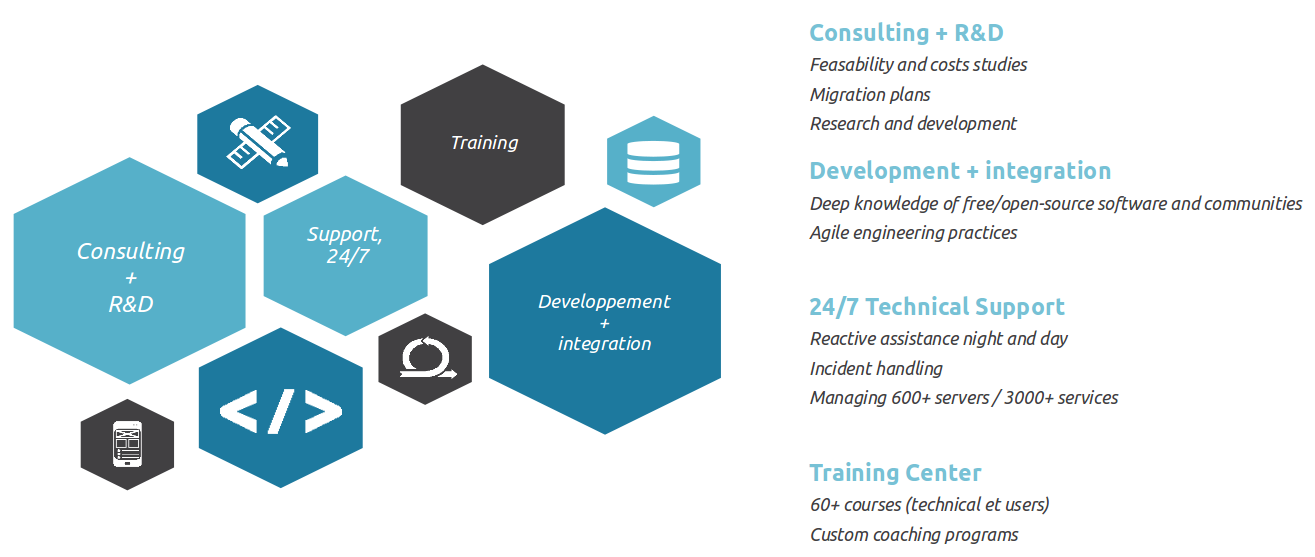
\includegraphics[width=11cm]{../pics/SFL-services}
	\end{figure}
\end{frame}

\frame{
	\frametitle{Triple Bottom Line}
	\begin{columns}[b]
		\column{0.3\textwidth}\center % Public Domain
		\begin{figure}
			
\includegraphics[width=3cm]{../pics/code-1839406_960_720}
		\end{figure}
		\small Excellence

		\column{0.3\textwidth}\center % Public Domain
		\begin{figure}
			
\includegraphics[width=3cm]{../pics/environmental-protection-683437_960_720}
		\end{figure}
		\small Environment

		\column{0.3\textwidth}\center % (C) Gargamello https://framasphere.org/posts/929977
		\begin{figure}
			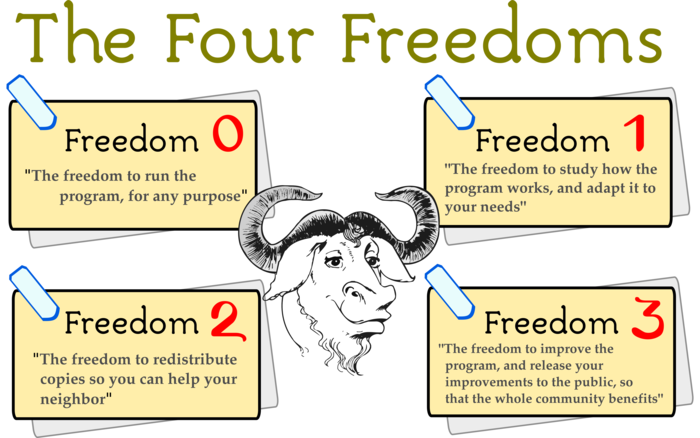
\includegraphics[width=3cm]{../pics/scaled_full_00c40105cea4c0aa3e9f}
		\end{figure}
		\small Community
	\end{columns}
}











% (C) Savoir-faire Linux, 2017 
% authored by Marc Lijour, March 2017 
% Some art belong to their respective authors, as indicated in the document
% 
% ======================================================================================================
%                                     FINTECH
% ======================================================================================================
\section{Insights on FinTech}
\frame{
	\begin{block}{}
		\begin{quote}
			{\Huge 20\% of the world's economy will be digital by 2020.} \\
			\vspace{1em}
			\hfill ---Accenture \#techvision2016
		\end{quote}
	\end{block}
}

\frame{
	\frametitle{FinTech: Technology resets the game for FSIs}
	\begin{itemize}
		\item ``Silicon Valley is coming'' ---Jamie Dimon, CEO, JP Morgan Chase
		\pause
		\item ``Half of the world's banks will disappear'' --- Francisco Gonzalez, Chief Executive, BBVA \vspace{2em}
		\pause
		\item Bitcoin $\rightarrow$ almost free remittances, cashless society?
		\pause
		\item Lending Club $\rightarrow$ individual to individual, shortcircuiting the bank
		\pause
		\item Wealthsimple $\rightarrow$ intelligent investment, Bye bye management fees
		\pause
		\item Square, Venmo $\rightarrow$ payment on the go
		\item etc
	\end{itemize}
}

\frame{
	\frametitle{The Milenials}
	\begin{figure} % https://www.flickr.com/photos/statefarm/26663820390
		
\includegraphics[width=11cm]{../pics/statefarm-milenials-CC-BY}
	\end{figure}
	\tiny \copyright \href{https://www.flickr.com/photos/statefarm/26663820390}{State Farm} (CC-BY license)
}

\begin{frame}
	\frametitle{Open Source runs (almost) Everything}
	\framesubtitle{2015 was an inflexion point}
	\begin{figure} % extracts from articles and other sources published on the Web
		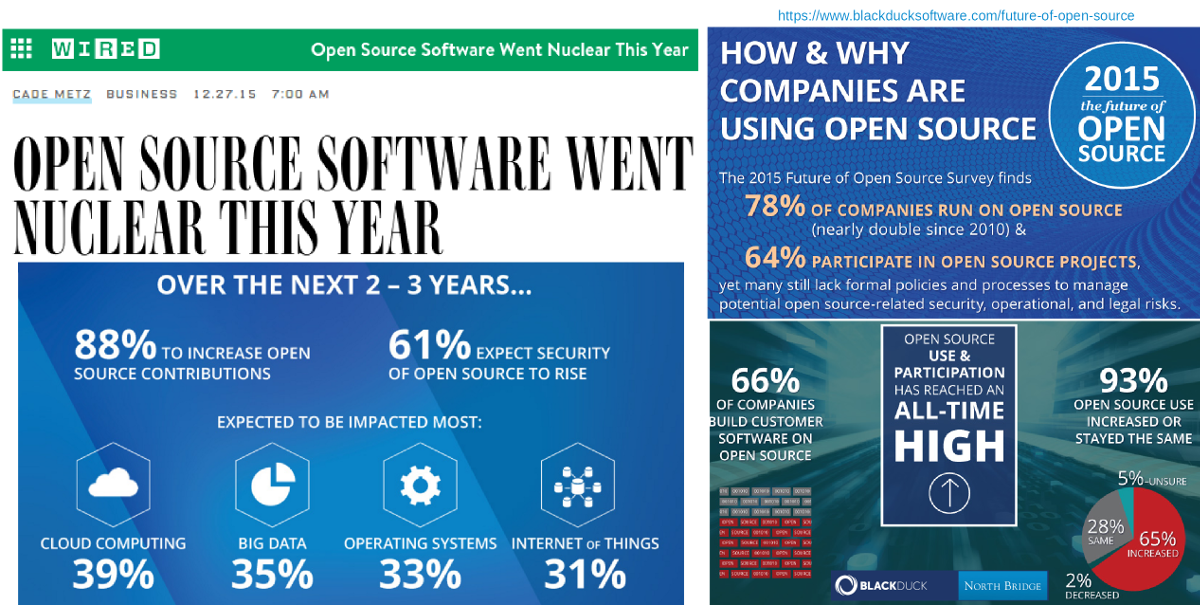
\includegraphics[width=11cm]{../pics/pic-open-source-went-nuclear-non-interlaced}
	\end{figure}
\end{frame}

\frame{
	\frametitle{A threatening Gap for Incubants}
	\begin{columns}[t]
		\column{0.5\textwidth}
		{\center Start ups}
		\begin{itemize}
			\item Small
			\item Agile
			\item Open Source
			\item Bootstrapping
		\end{itemize}
		
		\column{0.5\textwidth}
		{\center Old Bank} 
		\begin{itemize}
			\item Very large (often dealing with multiple jurisdictions)
			\item Siloed and burdened with processes
			\item Legacy technology (mainframe, COBOL, etc)
			\item Supporting a branch network (brick and mortar)
		\end{itemize}
		
	\end{columns}
}

\frame{
	\frametitle{Areas of Focus for Financial Services Institutions (FSIs)}
	\begin{columns}
		\column{0.3\textwidth}\center
		\begin{figure}
			
\includegraphics[width=1.5cm]{../pics/icons/headphones-8x}
		\end{figure}
		\tiny Reduce Customer Friction

		\column{0.3\textwidth}\center
		\begin{figure}
			
\includegraphics[width=1.5cm]{../pics/icons/droplet-8x}
		\end{figure}
		\tiny Save on Costs

		\column{0.3\textwidth}\center
		\begin{figure}
			
\includegraphics[width=1.5cm]{../pics/icons/graph-8x}
		\end{figure}
		\tiny Generate New Revenues

	\end{columns}
}

\frame{
	\frametitle{Technology Tsunami in Progress}
	\framesubtitle{\ldots and as many job opportunities\ldots}
	\begin{itemize}
		\item DevOps $\rightarrow$ BizDevOps
		\pause
		\item Blockchain 
		\pause
		\item Big Data and Analytics (Hadoop is hot)
		\pause
		\item Artificial Intelligence, Machine Learning 
	\end{itemize}
}

\frame{
	\frametitle{The Challenge for FSIs}
	\begin{block}{}
		\begin{quote}
			{\Huge To generate relevant and valuable services for the customer, as expectations rise, \\
			and to do it fast enough.} \\
		\end{quote}
	\end{block}
}


% (C) Savoir-faire Linux, 2017 
% authored by Marc Lijour, March 2017 
% Some art belong to their respective authors, as indicated in the document
% 
% ======================================================================================================
%                                      CASE STUDY
% ======================================================================================================
\section{Desjardins Case Study}
\frame{
	\frametitle{Our mission was to help Customer-Facing Employees to be more productive}
	\framesubtitle{The 45,000 ``Conseillers Desjardins''} 
	\begin{figure}	
		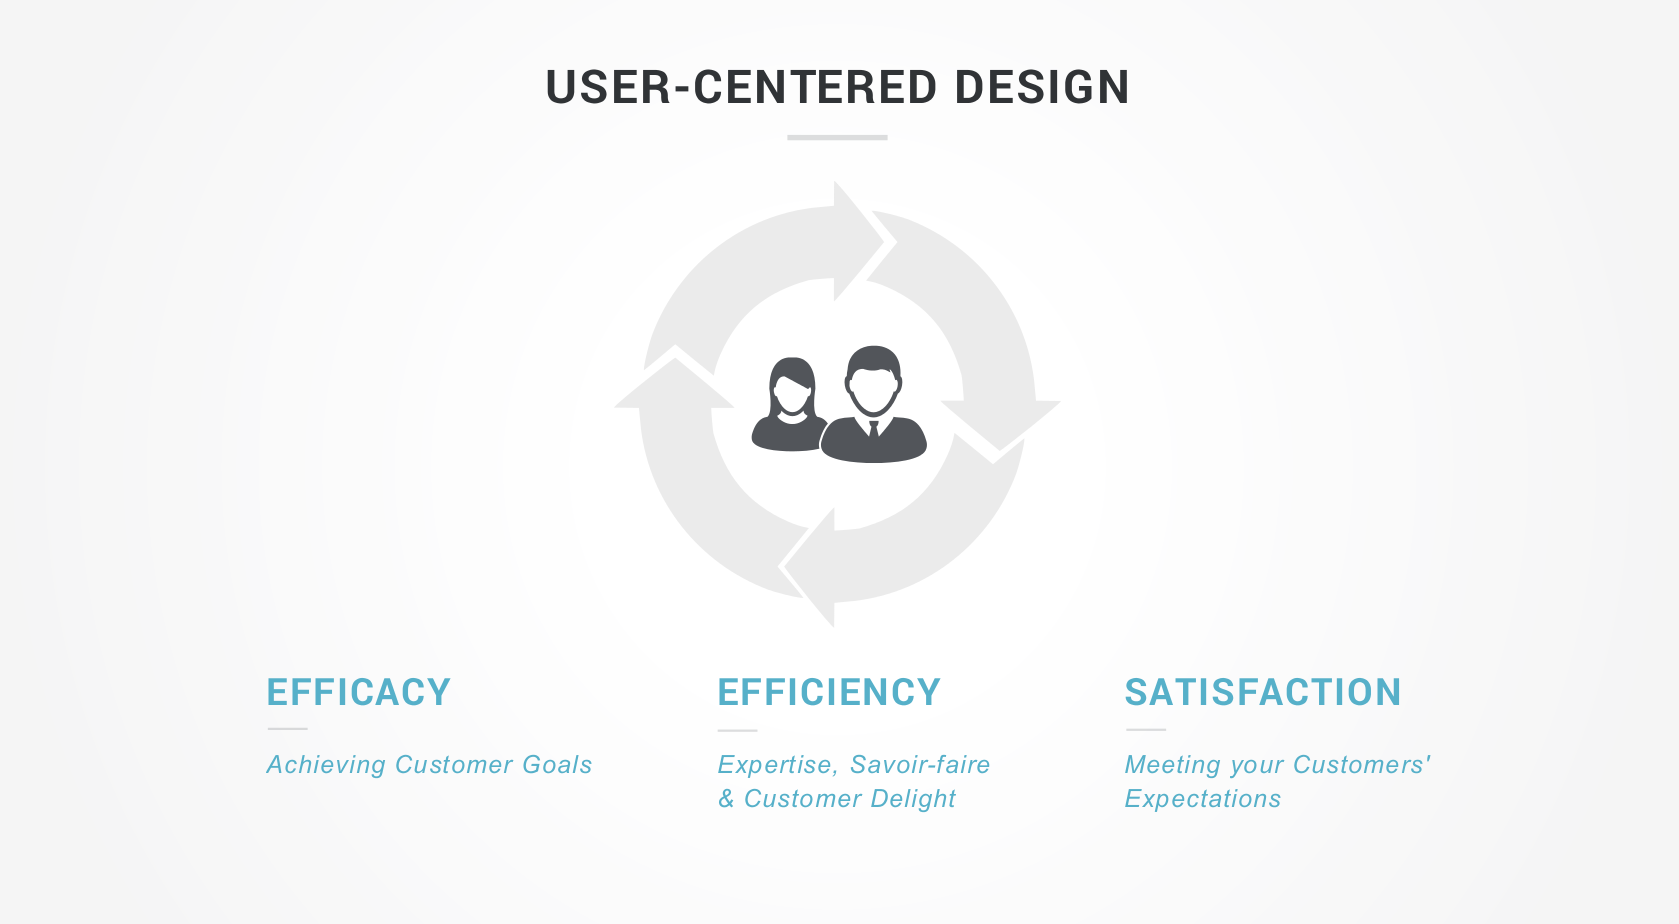
\includegraphics[width=11cm]{../pics/user-centered-design}
	\end{figure}
}

\frame{
	\frametitle{BizDevOps in Action}
	\framesubtitle{Developers work Closely with the Customers and End-Users}
	\begin{figure}	
		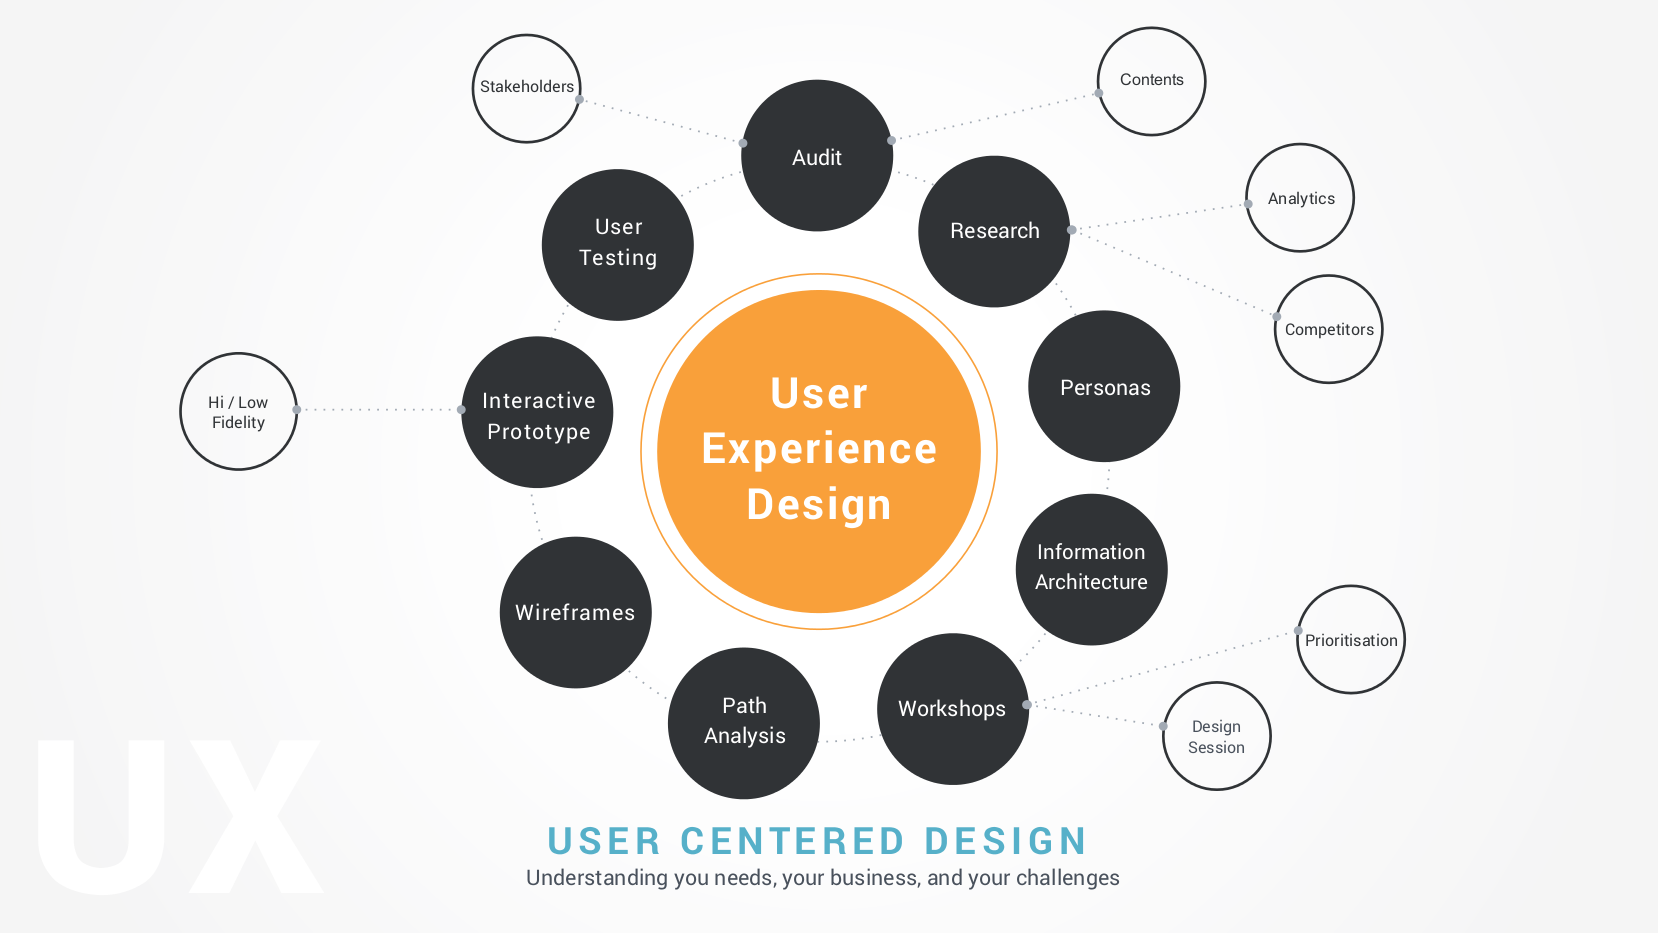
\includegraphics[width=11cm]{../pics/user-centered-design-process}
	\end{figure}
}

\frame{
	\frametitle{Bring the most value for each type of user}
	\begin{figure}	
		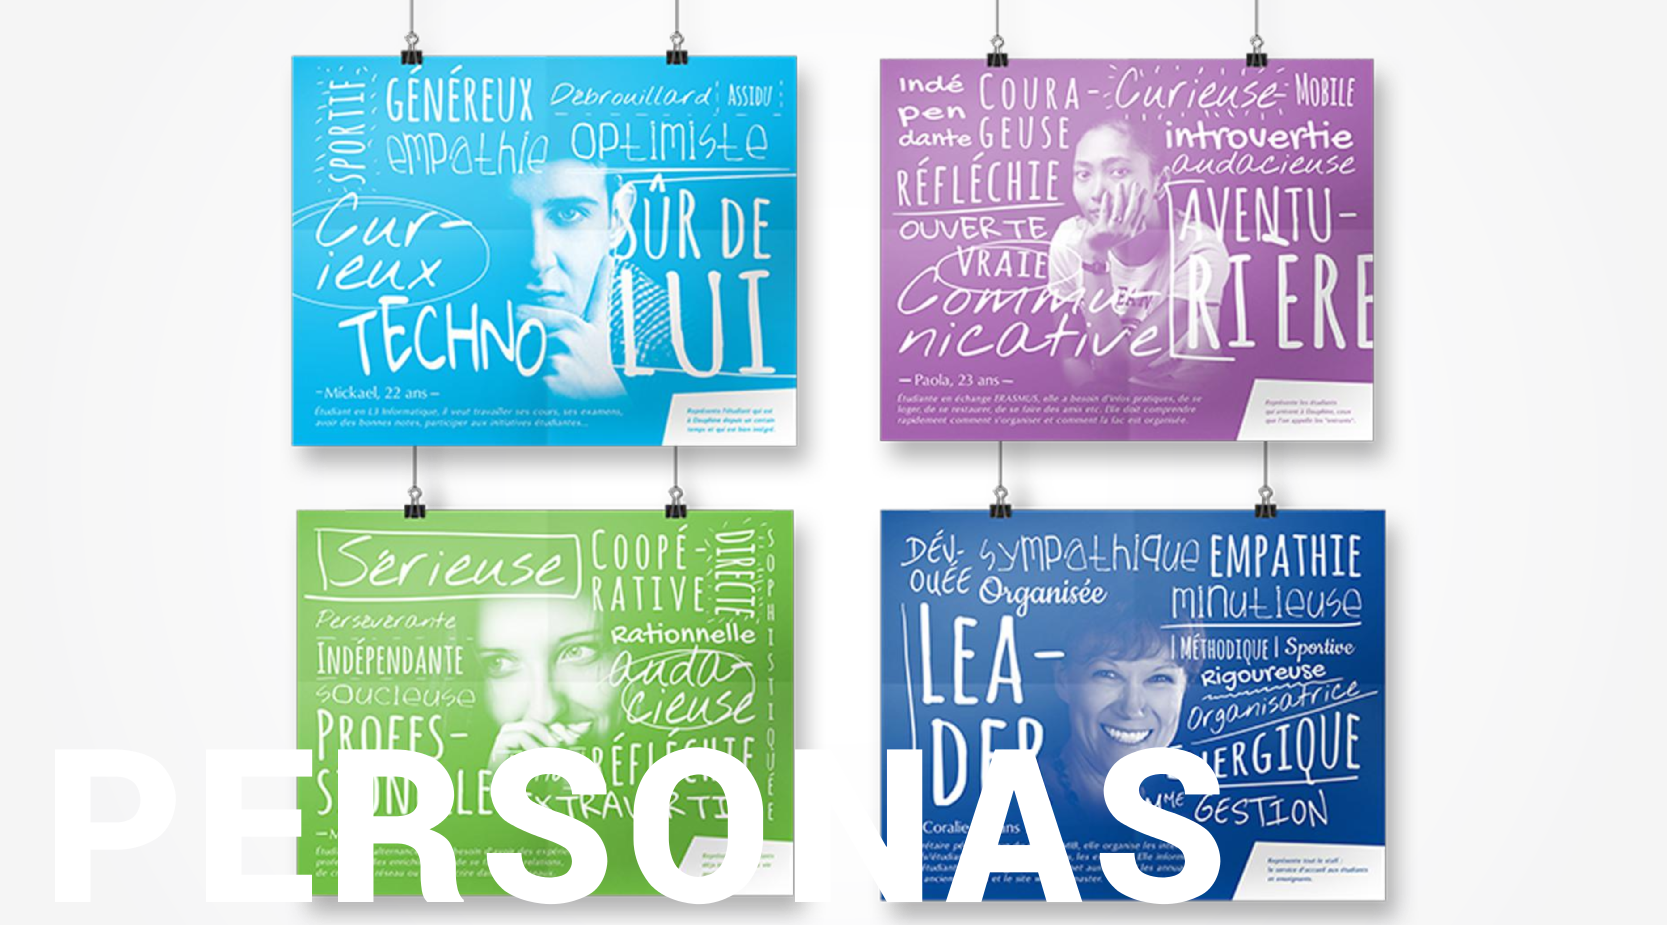
\includegraphics[width=11cm]{../pics/personas}
	\end{figure}
}

\frame{
	\frametitle{Liferay is a perfect choice for FSIs}
	\framesubtitle{Java-based, Enterprise-Ready, Open Source, Local Partners to help}
	\begin{figure}	
		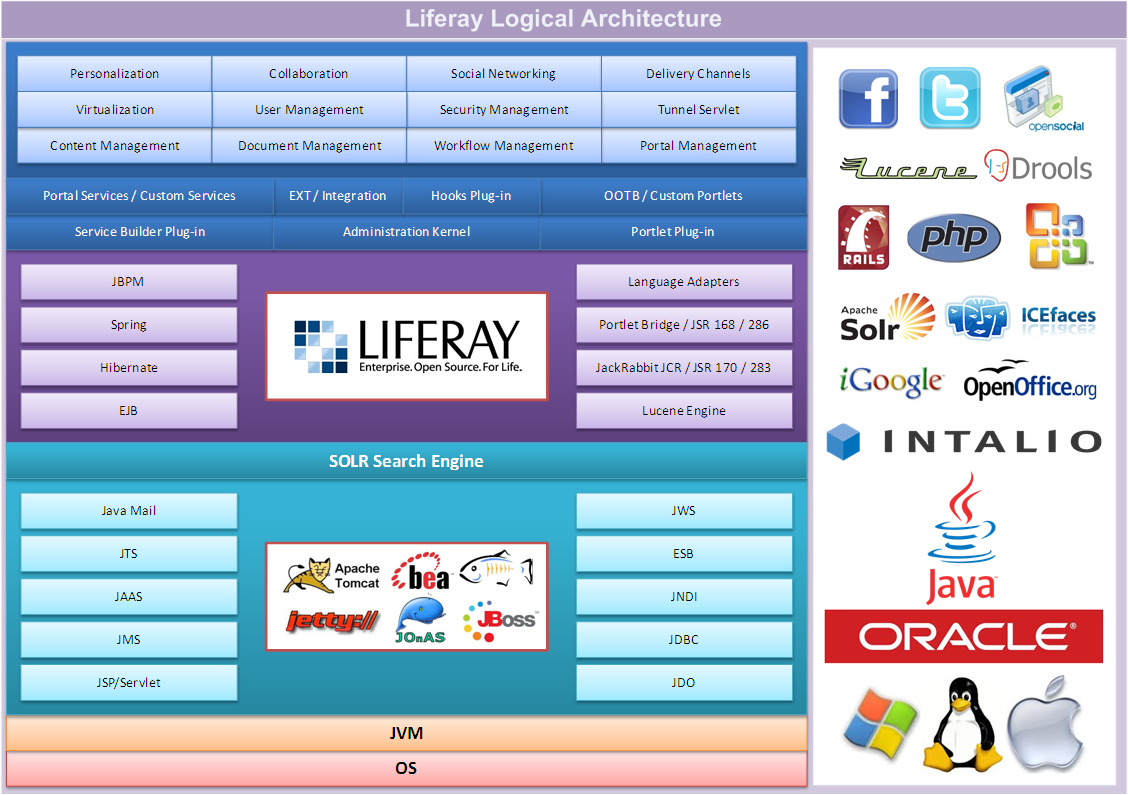
\includegraphics[width=11cm]{../pics/liferay-logical-architecture}
	\end{figure}
}

\frame{
	\frametitle{Concept}
	\begin{figure}	
		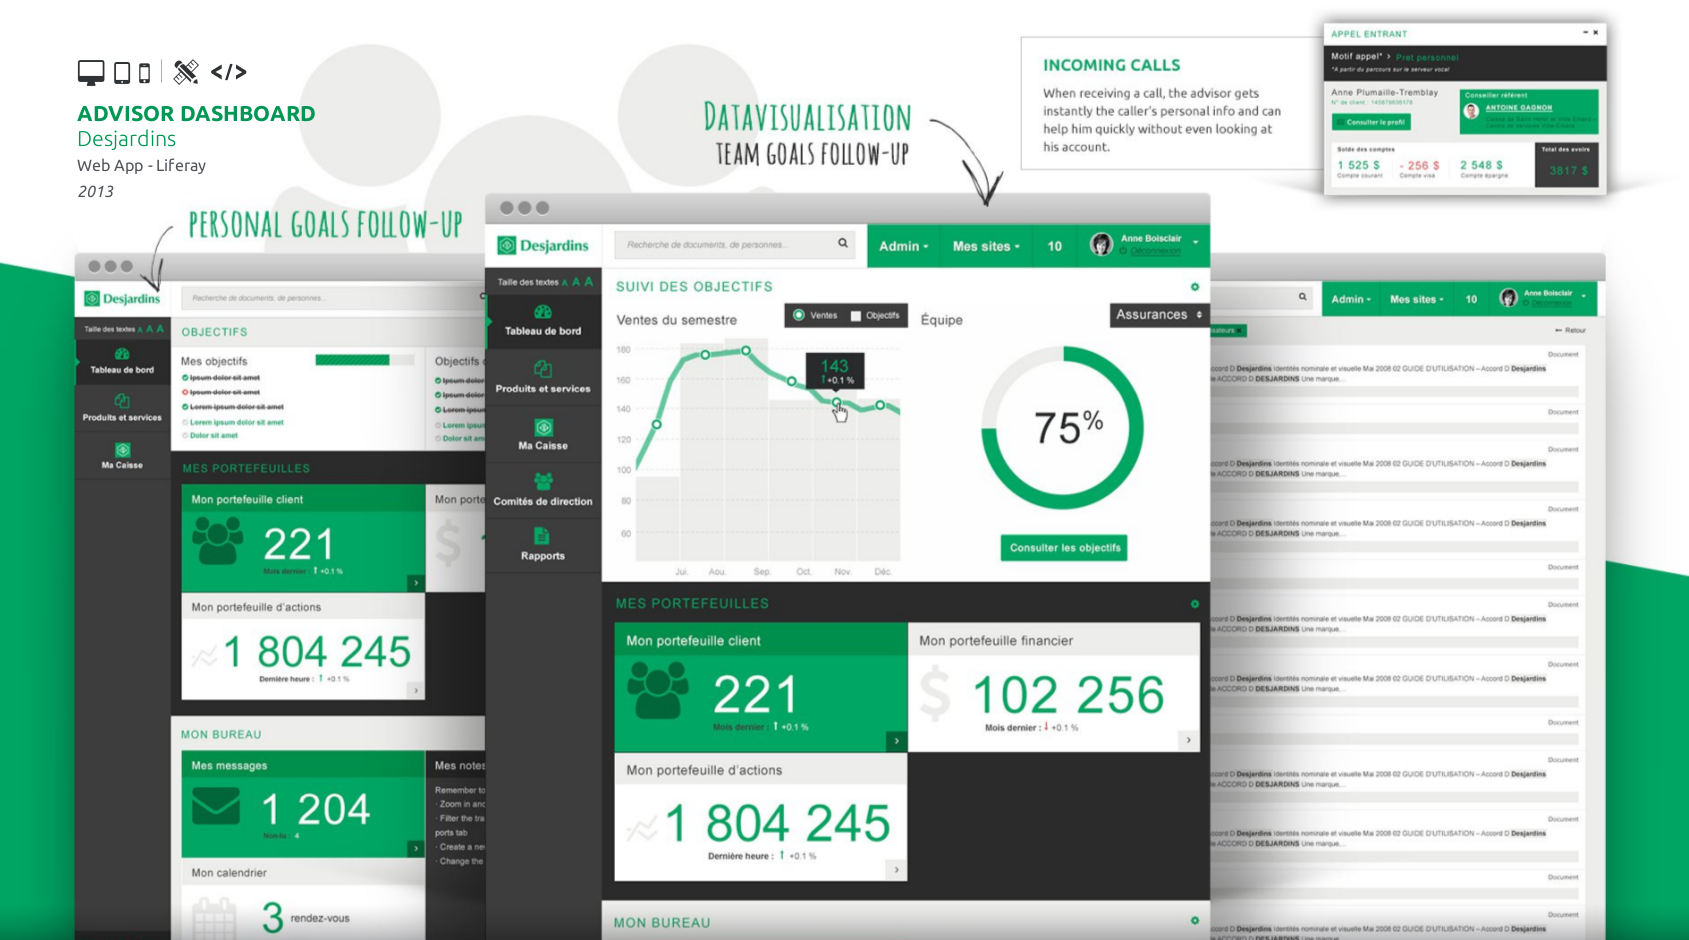
\includegraphics[width=11cm]{../pics/desjardins-concept}
	\end{figure}
}


% (C) Savoir-faire Linux, 2017 
% authored by Marc Lijour, Maxim Gorshkov, March 2017 
% Some art belong to their respective authors, as indicated in the document
% 
% ======================================================================================================
%                                      WORKSHOP
% ======================================================================================================
\section{Worshop}
\frame{
	\frametitle{Workshop}
	\framesubtitle{Developing an app for an online insurance}
	The \href{https://github.com/mkgorshkov/Ryerson_Presentation_March15/blob/master/slides/RyersonUniversityPresentationMarch15.pdf}{workshop} will focus on Liferay, a sophisticated Content Management System (CMS), built on Java, that makes it easy to design, develop, and implement modern applications. Attendees will practice with building an app for a fictitious auto insurance company, using Liferay and Vaadin.\\
	\vspace{1em}
	Maxim Gorshkov has prepared two sets of documents, \emph{i)} skeleton app to fill in the blanks, and \emph{ii)} a complete solution, respectively:
	\begin{itemize}\footnotesize
		\item \url{https://github.com/mkgorshkov/Ryerson_Presentation_March15_Learning}
		\item \url{https://github.com/mkgorshkov/Ryerson_Presentation_March15}
	\end{itemize}
	\vspace{1em}
	The winner gets a Savoir-faire Linux Tee-Shirt and a shot at a Summer Internship!
}


% (C) Savoir-faire Linux, 2017 
% authored by Marc Lijour, March 2017 
% Some art belong to their respective authors, as indicated in the document
% 
% ======================================================================================================
%                                      CLOSING
% ======================================================================================================
\section{Thanks}
\frame{
	\frametitle{Special Thanks to our Sponsors}
	\begin{columns}
		\column{0.3\textwidth}
		\begin{figure}
			
\includegraphics[width=2.5cm]{../../Savoir-faire_Linux-LaTeX_Templates/images/logo-sfl-250}
		\end{figure}
		
		\column{0.3\textwidth}
		\begin{figure}
			
\includegraphics[width=4cm]{../pics/logos/Liferay_logo-large-640x183}
		\end{figure}
		
		\column{0.3\textwidth}
		\begin{figure}
			
\includegraphics[width=3cm]{../pics/logos/ovh-square}
		\end{figure}
		
	\end{columns}
}

\frame{
	\begin{block}{Contact Information}\center
		\href{mailto:Marc.Lijour@savoirfairelinux.com}{Marc.Lijour@savoirfairelinux.com}\\
		\href{https://twitter.com/marclijour}{Twitter}: @marclijour\\
		\href{https://ring.cx}{Ring me}: marclijour
	\end{block}
}


\end{document}

